\documentclass[10pt]{beamer}

\usepackage{amsmath}
\usepackage{dsfont}
\usepackage{pgfplots}
\usepackage{pgfplotstable}
\usepackage{tikz}
\usepackage{xcolor}

\usetikzlibrary{arrows.meta}
\usetikzlibrary{calc}

\usetheme{PSY9511}

\title{PSY9511: Seminar 1}
\subtitle{Introduction to machine learning}
\author{Esten H. Leonardsen}
\date{\today}


\definecolor{full}{HTML}{ef476f}
\definecolor{bias}{HTML}{26547c}
\definecolor{variance}{HTML}{06d6a0}
\definecolor{train}{HTML}{ffd166}

\pgfplotsset{
    discard if not/.style 2 args={
        x filter/.code={
            \edef\tempa{\thisrow{#1}}
            \edef\tempb{#2}
            \ifx\tempa\tempb
            \else
                \def\pgfmathresult{inf}
            \fi
        }
    }
}

\begin{document}
	\begin{frame}
	 	\maketitle
	\end{frame}

    \begin{frame}{Outline}
        \textbf{Plan for the day}
        \begin{itemize}
            \item Round of introductions
            \item Course information
            \item Introduction to machine learning
            \item Presentation of assignment 1
        \end{itemize}
    \end{frame}

    % \begin{frame}{Teacher}
%     \textbf{Esten Høyland Leonardsen}
%     \begin{itemize}
%         \item Master's degree in Informatics: Programming and Networks
%         \item PhD in Psychology, deep learning applied to neuroimaging data
%         \item Experience as a data scientist and programmer from the industry and various start-ups
%         \item Post-doc at the center for Cognitive psychology, Neuroscience and Neuropsychology
%         \item Chief Scientific Officer at baba.vision
%         \item Interests: Deep learning, explainable artificial intelligence, mental health, neuroimaging
%     \end{itemize}
% \end{frame}

% \begin{frame}{Students}
%     \textbf{What I want to know about you}
%     \begin{itemize}
%         \item What's your name?
%         \item What department/section are you from?
%         \item What's your research project about?
%         \item Do you have experience with machine learning and/or programming?
%         \item What do you hope to learn from this course? (e.g. specific applications in your research, a theoretical understanding of machine learning, following and contributing to the public discourse, a future job in data science, ...)
%     \end{itemize}
% \end{frame}

% \begin{frame}{About the course}
%     \begin{tikzpicture}
%     \visible<1>{
%         \node[text width=10.5cm] at (0, 0) {
%             \textbf{Canvas}
%             \begin{itemize}
%                 \item All relevant announcements will be made on Canvas (e.g. changes to assignments, lectures, interesting reading material etc.)
%                 \item Lecture slides and notebooks from live coding will be put on Canvas before/after a lecture
%             \end{itemize}
%         };
%     }
%     \visible<2>{
%         \node[text width=10.5cm] at (0, 0) {
%             \textbf{Curriculum}
%             \begin{itemize}
%                 \item The course relies on the book "An Introduction to Statistical Learning", available at \url{https://www.statlearning.com/}
%                 \begin{itemize}
%                     \item Only some chapters will be used, they are posted on Canvas under each Lecture module
%                     \item Although we won't be relying much on the exercises i \textbf{highly recommend} looking into them yourselves
%                 \end{itemize}
%                 \item I will add some scientific publications to the curriculum list as we go, depending on your preferences and interests
%             \end{itemize}
%         };
%     }
%     \visible<3>{
%         \node[text width=10.5cm] at (0, 0) {
%             \textbf{Exercises}
%             \begin{itemize}
%                 \item The course has no exam, but six mandatory exercises you will need to pass
%                 \begin{itemize}
%                     \item Mostly practical coding, with some reflection
%                     \item Given with a \textbf{hard} deadline, unless there is a good reason for an extension
%                     \item Can be delivered multiple times based on feedback (but the first must be in time for the original deadline)
%                 \end{itemize}
%                 \item Exercises 1-4 and 6 are mostly small and related to specific content of the preceding lecture, while 5 is a bit larger
%                 \item You should hand in runnable code (e.g. a Jupyter notebook, a python script, an R script, Rmarkdown etc.), not code copied into a Word document or a pdf
%             \end{itemize}
%         };
%     }
%     \visible<4>{
%         \node[text width=10.5cm] at (0, 0) {
%             \textbf{Generative artificial intelligence (e.g. ChatGPT)}
%             \begin{itemize}
%                 \item You are allowed to use generative AI in the assignments, but you must state where and how
%                 \begin{itemize}
%                     \item Be critical, you should be able to understand and explain \textbf{all} the code you hand in
%                 \end{itemize}
%             \end{itemize}
%         };
%     }
%     \visible<5>{
%         \node[text width=10.5cm] at (0, 0) {
%             \textbf{Lectures}
%             \begin{itemize}
%                 \item Goal is to show you the underlying theory in an intuitive manner
%                 \item $\sim$2 hours of lecturing, $\sim$1 hour for individual work/help with assignments
%                 \begin{itemize}
%                     \item You will have to practice what you learn yourself
%                 \end{itemize}
%                 \item Will try to make lectures interactive, and do live coding where possible
%             \end{itemize}
%         };
%     }
%     \visible<6>{
%         \node[text width=10.5cm] at (0, 0) {
%             \textbf{Course plan}
%             \begin{enumerate}
%                 \item Introduction to machine learning
%                 \item Basics of regression and classification
%                 \item Variable selection and regularization
%                 \item Model selection, validation, and testing
%                 \item Non linearity: Splines and tree-based methods
%                 \item Unsupervised learning
%                 \item Deep learning and image processing
%                 \item Language processing
%             \end{enumerate}
%         };
%     }
%     \end{tikzpicture}
% \end{frame}

    \section{Introduction to machine learning}

\begin{frame}{Introduction}
    \begin{tikzpicture}
        \node[] at (-5.25, -3.5) {};
        \node[] at (5.25, 3.5) {};
        \visible<1-3>{
            \node[text width=10.5cm, align=flush left] at (0, 0) {
                \textbf{Key terminology:}
                \begin{itemize}
                    \item Statistical learning: A set of tools (often called models) for finding patterns in data.
                    \item<2-> Machine learning: Approximately the same as statistical learning.
                    \begin{itemize}
                        \item<2-> More common among practitioners with a computer science or engineering background.
                        \item<2-> Often has a focus on prediction (as opposed to understanding).
                        \item<2-> Often uses very large datasets.
                        \item<2-> More pragmatic in nature(?).
                    \end{itemize}
                    \item<3> Supervised learning: We know what task we want the model to solve.
                    \item<3> Unsupervised learning: We don't know what task we want the model to solve (or we don't have the data needed to solve it).
                \end{itemize}
            };
        }
        \visible<4-5,7-8>{

            \node[inner sep=0pt, draw=black, anchor=west] (x1) at (-5.25, 2.5) {
                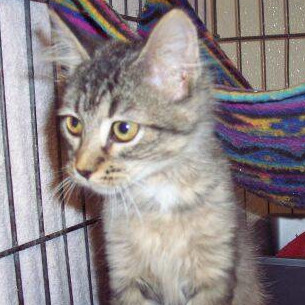
\includegraphics[width=1cm]{data/cats_and_dogs/cat.2.jpg}
            };
            \node[inner sep=0pt, draw=black] (x2) at ($ (x1) - (0, 1.5) $) {
                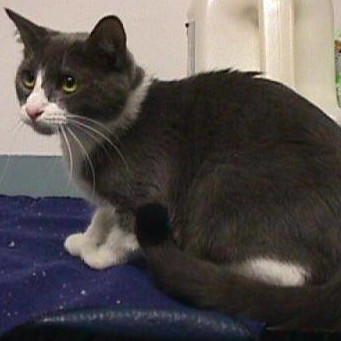
\includegraphics[width=1cm]{data/cats_and_dogs/cat.0.jpg}
            };
            \node[inner sep=0pt, draw=black] (x3) at ($ (x1) - (0, 3) $) {
                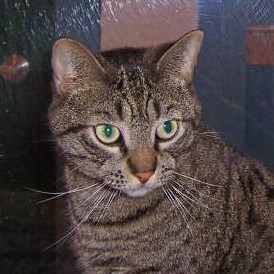
\includegraphics[width=1cm]{data/cats_and_dogs/cat.1.jpg}
            };
            \node[inner sep=0pt, draw=black] (x3) at ($ (x1) - (0, 4.5) $) {
                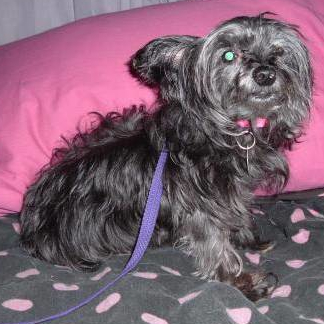
\includegraphics[width=1cm]{data/cats_and_dogs/dog.0.jpg}
            };

            \node[inner sep=0pt, draw=black] (x5) at ($ (x1) - (-1.25, 0.75) $) {
                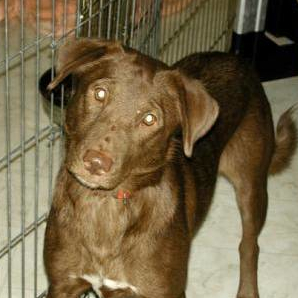
\includegraphics[width=1cm]{data/cats_and_dogs/dog.1.jpg}
            };
            \node[inner sep=0pt, draw=black] (x6) at ($ (x1) - (-1.25, 2.25) $) {
                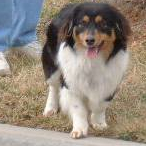
\includegraphics[width=1cm]{data/cats_and_dogs/dog.2.jpg}
            };
            \node[inner sep=0pt, draw=black] (x7) at ($ (x1) - (-1.25, 3.75) $) {
                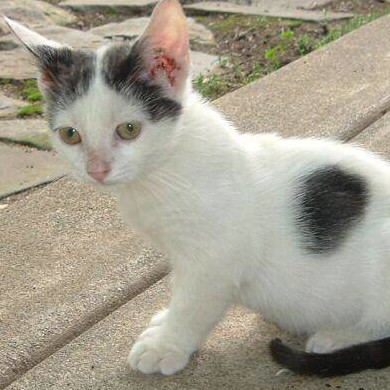
\includegraphics[width=1cm]{data/cats_and_dogs/cat.3.jpg}
            };
        }
        \visible<6>{
            \node[inner sep=0pt, draw=black, anchor=west, label=below:\tiny{Cat}] (x1) at (-5.25, 2.5) {
                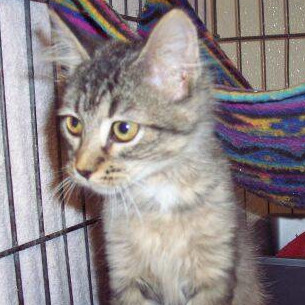
\includegraphics[width=1cm]{data/cats_and_dogs/cat.2.jpg}
            };
            \node[inner sep=0pt, draw=black, label=below:\tiny{Cat}] (x2) at ($ (x1) - (0, 1.5) $) {
                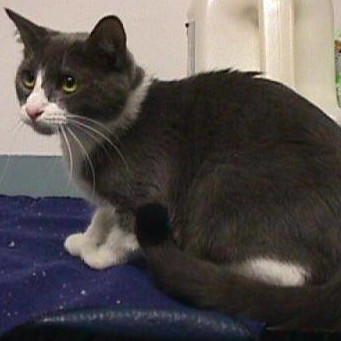
\includegraphics[width=1cm]{data/cats_and_dogs/cat.0.jpg}
            };
            \node[inner sep=0pt, draw=black, label=below:\tiny{Cat}] (x3) at ($ (x1) - (0, 3) $) {
                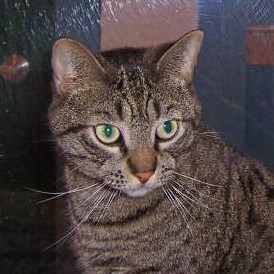
\includegraphics[width=1cm]{data/cats_and_dogs/cat.1.jpg}
            };
            \node[inner sep=0pt, draw=black, label=below:\tiny{Dog}] (x3) at ($ (x1) - (0, 4.5) $) {
                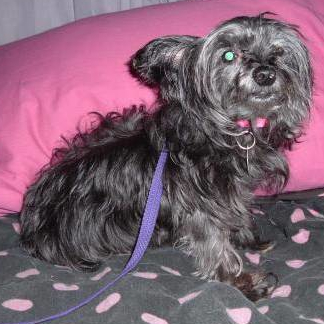
\includegraphics[width=1cm]{data/cats_and_dogs/dog.0.jpg}
            };

            \node[inner sep=0pt, draw=black, label=below:\tiny{Dog}] (x5) at ($ (x1) - (-1.25, 0.75) $) {
                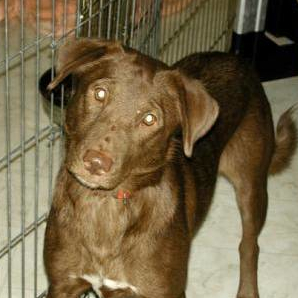
\includegraphics[width=1cm]{data/cats_and_dogs/dog.1.jpg}
            };
            \node[inner sep=0pt, draw=black, label=below:\tiny{Dog}] (x6) at ($ (x1) - (-1.25, 2.25) $) {
                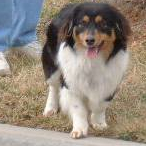
\includegraphics[width=1cm]{data/cats_and_dogs/dog.2.jpg}
            };
            \node[inner sep=0pt, draw=black, label=below:\tiny{Cat}] (x7) at ($ (x1) - (-1.25, 3.75) $) {
                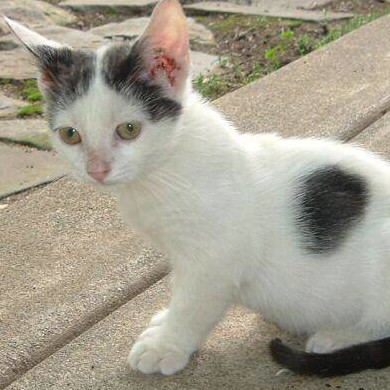
\includegraphics[width=1cm]{data/cats_and_dogs/cat.3.jpg}
            };
        }
        \visible<5-6,9>{
            \node[align=center, font=\scriptsize, draw=black] (sm) at ($ (x1) + (3.5, -0.75) $) {
                Supervised\\model
            };
        }
        \visible<5-6>{
            \draw[-stealth, gray!50, line width=3pt] (x6) to [in=270, out=0] (sm);
            \draw[-stealth, gray!50, line width=3pt] (sm) -- ($ (sm.east) + (1.1, 0) $);

            \node[inner sep=0pt, draw=black] (y1) at ($ (sm.center) + (5, 0.5) $) {
                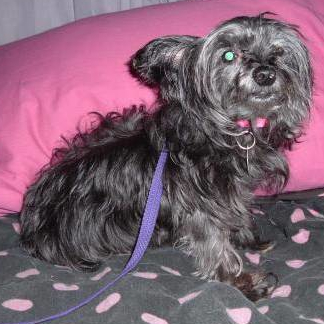
\includegraphics[width=1cm]{data/cats_and_dogs/dog.0.jpg}
            };
            \node[anchor=west, inner sep=0pt, draw=black] (y2) at (y1.east) {
                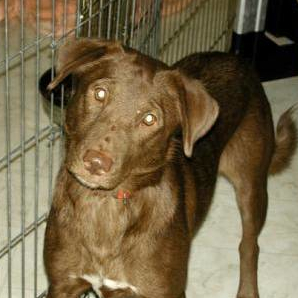
\includegraphics[width=1cm]{data/cats_and_dogs/dog.1.jpg}
            };
            \node[anchor=north, inner sep=0pt, draw=black] at (y1.south) {
                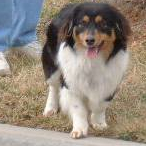
\includegraphics[width=1cm]{data/cats_and_dogs/dog.2.jpg}
            };

            \node[inner sep=0pt, draw=black] (y4) at ($ (sm) + (2.5, 0.5) $) {
                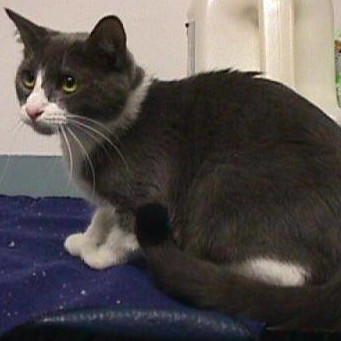
\includegraphics[width=1cm]{data/cats_and_dogs/cat.0.jpg}
            };
            \node[anchor=west, inner sep=0pt, draw=black] (y5) at (y4.east) {
                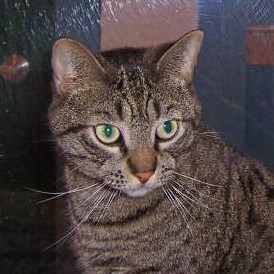
\includegraphics[width=1cm]{data/cats_and_dogs/cat.1.jpg}
            };
            \node[anchor=north, inner sep=0pt, draw=black] (y6) at (y4.south) {
                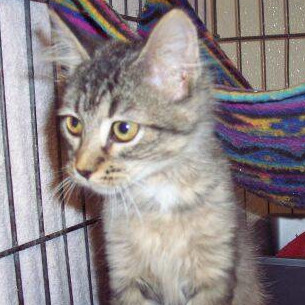
\includegraphics[width=1cm]{data/cats_and_dogs/cat.2.jpg}
            };
            \node[anchor=north, inner sep=0pt, draw=black] (y7) at (y5.south) {
                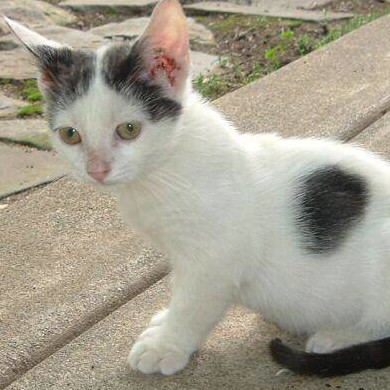
\includegraphics[width=1cm]{data/cats_and_dogs/cat.3.jpg}
            };

            \node[anchor=south, text depth=0] at ($ (y1.north)!0.5!(y2.north) $) {
                Dogs
            };
            \node[anchor=south, text depth=0] at ($ (y4.north)!0.5!(y5.north) $) {
                Cats
            };
        }
        \visible<7-9>{
            \node[align=center, font=\scriptsize, draw=black] (um) at ($ (x1) + (3.5, -3.75) $) {
                Unsupervised\\model
            };
        }
        \visible<7-8>{

            \draw[-stealth, gray!50, line width=3pt] (x6) to [in=90, out=0] (um);
            \draw[-stealth, gray!50, line width=3pt] (um) -- ($ (um.east) + (1.1, 0) $);
        }
        \visible<7>{
            \node[inner sep=0pt, draw=black] at ($ (um.center) + (6, 0.55) $) {
                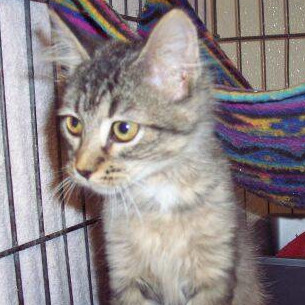
\includegraphics[width=1cm]{data/cats_and_dogs/cat.2.jpg}
            };
            \node[inner sep=0pt, draw=black] at ($ (um.center) + (5.95, -0.65) $) {
                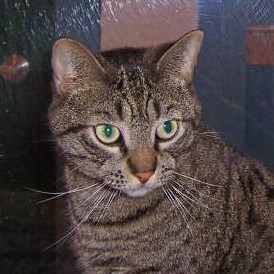
\includegraphics[width=1cm]{data/cats_and_dogs/cat.1.jpg}
            };
            \node[inner sep=0pt, draw=black] at ($ (um.center) + (4.8, 0.4) $) {
                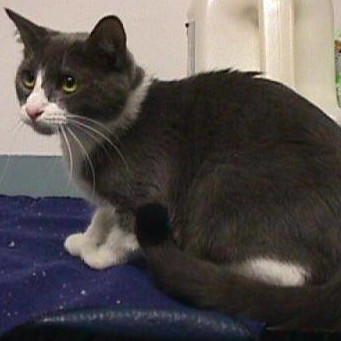
\includegraphics[width=1cm]{data/cats_and_dogs/cat.0.jpg}
            };
            \node[inner sep=0pt, draw=black] at ($ (um.center) + (4.7, -0.7) $) {
                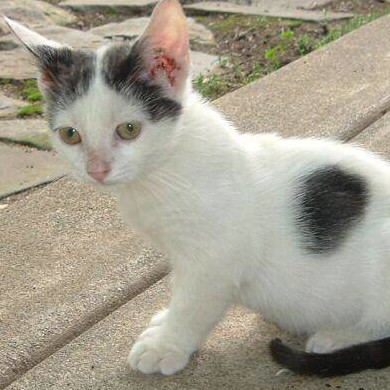
\includegraphics[width=1cm]{data/cats_and_dogs/cat.3.jpg}
            };

            \node[inner sep=0pt, draw=black] at ($ (um.center) + (2.7, 1.2) $) {
                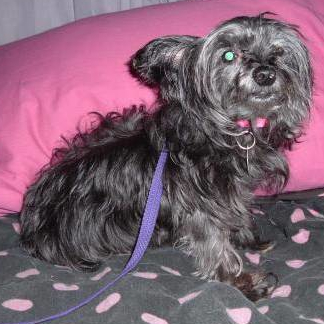
\includegraphics[width=1cm]{data/cats_and_dogs/dog.0.jpg}
            };
            \node[inner sep=0pt, draw=black] at ($ (um.center) + (2.55, 0) $) {
                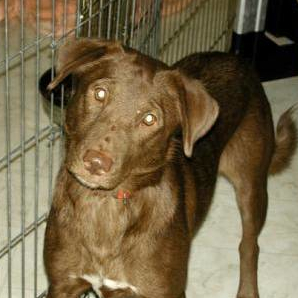
\includegraphics[width=1cm]{data/cats_and_dogs/dog.1.jpg}
            };
            \node[inner sep=0pt, draw=black] at ($ (um.center) + (2.65, -1.1) $) {
                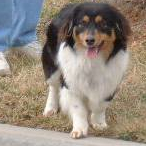
\includegraphics[width=1cm]{data/cats_and_dogs/dog.2.jpg}
            };
        }
        \visible<8>{
            \node[inner sep=0pt, draw=black] at ($ (um.center) + (6, 0.55) $) {
                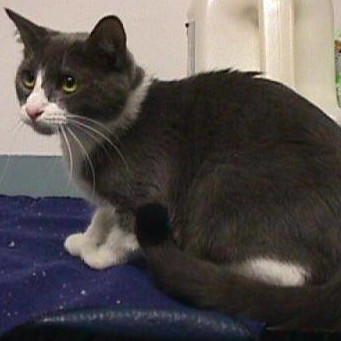
\includegraphics[width=1cm]{data/cats_and_dogs/cat.0.jpg}
            };
            \node[inner sep=0pt, draw=black] at ($ (um.center) + (5.95, -0.65) $) {
                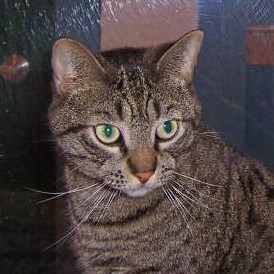
\includegraphics[width=1cm]{data/cats_and_dogs/cat.1.jpg}
            };
            \node[inner sep=0pt, draw=black] at ($ (um.center) + (4.8, 0.4) $) {
                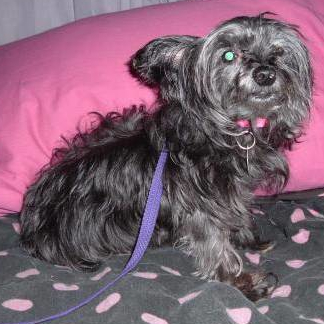
\includegraphics[width=1cm]{data/cats_and_dogs/dog.0.jpg}
            };
            \node[inner sep=0pt, draw=black] at ($ (um.center) + (4.7, -0.7) $) {
                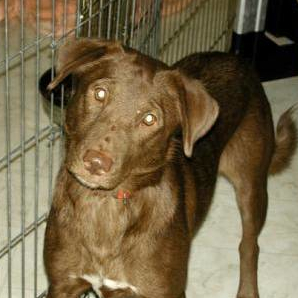
\includegraphics[width=1cm]{data/cats_and_dogs/dog.1.jpg}
            };

            \node[inner sep=0pt, draw=black] at ($ (um.center) + (2.7, 1.2) $) {
                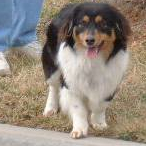
\includegraphics[width=1cm]{data/cats_and_dogs/dog.2.jpg}
            };
            \node[inner sep=0pt, draw=black] at ($ (um.center) + (2.55, 0) $) {
                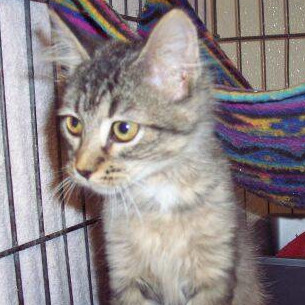
\includegraphics[width=1cm]{data/cats_and_dogs/cat.2.jpg}
            };
            \node[inner sep=0pt, draw=black] at ($ (um.center) + (2.65, -1.1) $) {
                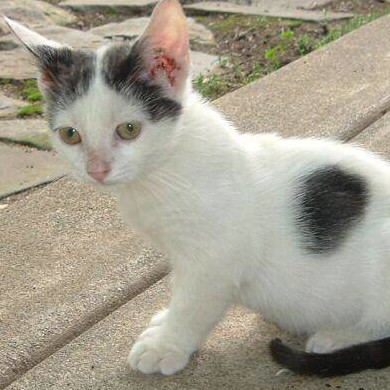
\includegraphics[width=1cm]{data/cats_and_dogs/cat.3.jpg}
            };
        }

    \end{tikzpicture}
\end{frame}

\newcommand{\mpgvsweight}[1]{
    \begin{tikzpicture}
        \begin{axis}[
            height=4cm,
            width=10cm,
            xlabel=$x$ (horsepower),
            ylabel=$y$ (mpg),
            ytick pos=left,
            xtick pos=bottom,
            xmin=30,
            xmax=245,
            ymin=6,
            ymax=51
        ]

        \addplot[
            only marks,
            cyan,
            opacity=0.5
        ] table [
            col sep=comma,
            x=horsepower,
            y=mpg
        ] {data/Auto.csv};

        \ifnum#1=1
            \draw[very thick, red] (axis cs: 30, 39-0.157*30) -- (axis cs: 245, 39-0.157*245);
            \node[text=red] at (axis cs: 180, 42) {
                $\hat{f}(x) = 39 - 0.157x$
            };
        \fi
        \ifnum#1=2
            \addplot[very thick, red, domain=30:245, samples=1000] {0.0012*x^2-0.46*x+56};
            \node[text=red] at (axis cs: 180, 42) {
                $\hat{f}(x) = 56+0.0012x^2-0.46x$
            };
        \fi
        \ifnum#1=3
            \addplot[very thick, red, smooth] coordinates {
                (6.0, 243.2069751806266)
                (15.958333333333334, 118.86132183998052)
                (25.916666666666668, 55.54830308937471)
                (35.875, 33.03657403682814)
                (45.833333333333336, 31.094789790600284)
                (55.79166666666667, 32.62203312809545)
                (65.75, 32.322995894942245)
                (75.70833333333334, 26.789726618159705)
                (85.66666666666667, 25.56443372228785)
                (95.625, 23.411114113578773)
                (105.58333333333334, 21.972291293527256)
                (115.54166666666667, 22.0202279029072)
                (125.5, 19.623191768387127)
                (135.45833333333334, 17.796535374305538)
                (145.41666666666669, 15.42464063855285)
                (155.375, 13.83975395598323)
                (165.33333333333334, 13.58266973340266)
                (175.29166666666669, 14.577234897250934)
                (185.25, 13.44873671948327)
                (195.20833333333334, 11.13569858732588)
                (205.16666666666669, 10.948027264126887)
                (215.125, 12.746078206932541)
                (225.08333333333334, 14.710541046885707)
                (235.04166666666669, 16.775438769652766)
                (245.0, 18.301538120974897)
            };
            \node[text=red] at (axis cs: 180, 42) {
                $\hat{f}(x) = \ldots$
            };
        \fi
        \ifnum#1>3
            \draw[very thick, red] (axis cs: 30, 39-0.157*30) -- (axis cs: 245, 39-0.157*245);
        \fi
        \ifnum#1=4
            \node[minimum height=0.4cm, minimum width=1.15cm, draw=black, very thick] at (axis cs: 197, 42) {};

            \node[text=red] at (axis cs: 180, 42) {
                $\hat{f}(x) = 39 - 0.157x$
            };
        \fi
        \ifnum#1>4
            \addplot[
                only marks,
                red,
                opacity=0.5
            ] coordinates {
                (125, 19.3)
            };
            \node[text=red, anchor=north] at (axis cs: 180, 48.4) {
                $\begin{aligned}
                \hat{f}(125) &= 39 - 0.157*125\\[-0.25cm]
                &= 19.3
                \end{aligned}$
            };
        \fi
        \ifnum#1>5
            \node[text=red] (yhat) at (axis cs: 176.5, 22) {
                $\hat{y}$
            };
            \draw[-stealth, red] (yhat.north) -- ($ (yhat.north) +( 0, 50) $);
        \fi

        \end{axis}
    \end{tikzpicture}
}

\newsavebox{\mpgpoints}
\sbox{\mpgpoints}{
    \mpgvsweight{0}
}
\newsavebox{\mpglinear}
\sbox{\mpglinear}{
    \mpgvsweight{1}
}
\newsavebox{\mpgsquared}
\sbox{\mpgsquared}{
    \mpgvsweight{2}
}
\newsavebox{\mpgnonparametric}
\sbox{\mpgnonparametric}{
    \mpgvsweight{3}
}
\newsavebox{\mpglinearhighlight}
\sbox{\mpglinearhighlight}{
    \mpgvsweight{4}
}
\newsavebox{\mpgcalculation}
\sbox{\mpgcalculation}{
    \mpgvsweight{5}
}
\newsavebox{\mpgyhat}
\sbox{\mpgyhat}{
    \mpgvsweight{6}
}

\begin{frame}{Introduction: Supervised learning}
    \begin{tikzpicture}
        \node[] at (-5.25, -3.5) {};
        \node[] at (5.25, 3.5) {};

        \visible<1-5>{
            \node[anchor=north west, ampersand replacement=\&, font=\footnotesize] at (-5.25, 3.5) {
                \begin{tabular}{|c|c|c|c|c|c|}
                    \hline
                    \textbf{name}&\alert<4>{\textbf{year}}&\alert<4>{\textbf{cylinders}}&\alert<4>{\textbf{horsepower}}&\alert<4>{\textbf{weight}}&\alert<3>{\textbf{mpg}}\\
                    \hline
                    Chevrolet Chevelle Malibu&\alert<4>{1970}&\alert<4>{8}&\alert<4>{130}&\alert<4>{3504}&\alert<3>{18}\\
                    \alert<2>{Buick Skylark 320}&\alert<2,4>{1980}&\alert<2,4>{4}&\alert<2,4>{165}&\alert<2,4>{3693}&\alert<2,3>{15}\\
                    Plymouth Satellite&\alert<4>{1971}&\alert<4>{8}&\alert<4>{150}&\alert<4>{3436}&\alert<3>{18}\\
                    AMC Rebel SST&\alert<4>{1975}&\alert<4>{4}&\alert<4>{150}&\alert<4>{3433}&\alert<3>{16}\\
                    Ford Torino&\alert<4>{1978}&\alert<4>{8}&\alert<4>{140}&\alert<4>{3449}&\alert<3>{17}\\
                    \hline
                \end{tabular}
            };
            \node[anchor=south west, text width=10.5cm] at (-5.25, -3.5) {
                \textbf{Prerequisites}
                \begin{itemize}
                    \item A dataset representing a given population
                    \item<3-> A response-variable $y$ that we want to predict
                    \item<4-> A set of predictors $X$ that we can use to predict $y$
                    \item<5-> An \textbf{assumed} relationship between $X$ and $y$ that can be described by an unknown function $f$, such that $y=f(X) + \epsilon$
                \end{itemize}
            };
        }
        \visible<6>{
            \node[] at (0, 1.75) {
                \usebox{\mpgpoints}
            };
        }
        \visible<7,9,11,13,15>{
            \node[] at (0, 1.75) {
                \usebox{\mpglinear}
            };
        }
        \visible<8,14>{
            \node[] at (0, 1.75) {
                \usebox{\mpgsquared}
            };
        }
        \visible<10>{
            \node[] at (0, 1.75) {
                \usebox{\mpgnonparametric}
            };
        }
        \visible<6-10>{
            \node[anchor=north west, text width=10.5cm] at (-5.25, 0) {
                \textbf{Estimation (or training the model)}
                \begin{itemize}
                    \item We have assumed that $y=f(X) + \epsilon$, but don't know $f$
                    \item<7-> We produce an estimate $\hat{f}$
                    \item<9-> Parametric models: $\hat{f}$ has a simple form
                    \begin{itemize}
                        \item<9-> $\hat{f}(x) = {\color{red}\beta_0} + {\color{red}\beta_1} x$
                    \end{itemize}
                    \item<10-> Non-parametric models: $\hat{f}$ relies directly on the data
                \end{itemize}
            };
        }
        \visible<12>{
           \node[] at (0, 1.75) {
               \usebox{\mpglinearhighlight}
           };
        }
        \visible<11-17>{
            \node[anchor=north west, text width=10.5cm, align=flush left] (inference) at (-5.25, 0) {
                \textbf{Inference: Understanding the relationship between the predictors and the response}
                \begin{itemize}
                    \item<12-> How does individual features relate to the response?
                    \item<13-> What is the \textit{functional form} of the relationship?
                \end{itemize}
            };
        }
        \visible<15-17>{
            \node[anchor=north west, text width=10.5cm, align=flush left] at (inference.south west) {
                \textbf{Prediction: Predicting the response for new observations}
                \begin{itemize}
                    \item Plugging new values $X$ into $\hat{f}(X)$
                \end{itemize}
            };
        }
        \visible<16>{
            \node[] at (0, 1.75) {
                \usebox{\mpgcalculation}
            };
        }
        \visible<17>{
            \node[] at (0, 1.75) {
                \usebox{\mpgyhat}
            };
        }
        \visible<18>{
            \node[] at (0, 0) {
                \url{http://localhost:8888/tree}
            };
        }
    \end{tikzpicture}
\end{frame}

\begin{frame}{Introduction: Functional interfaces}
    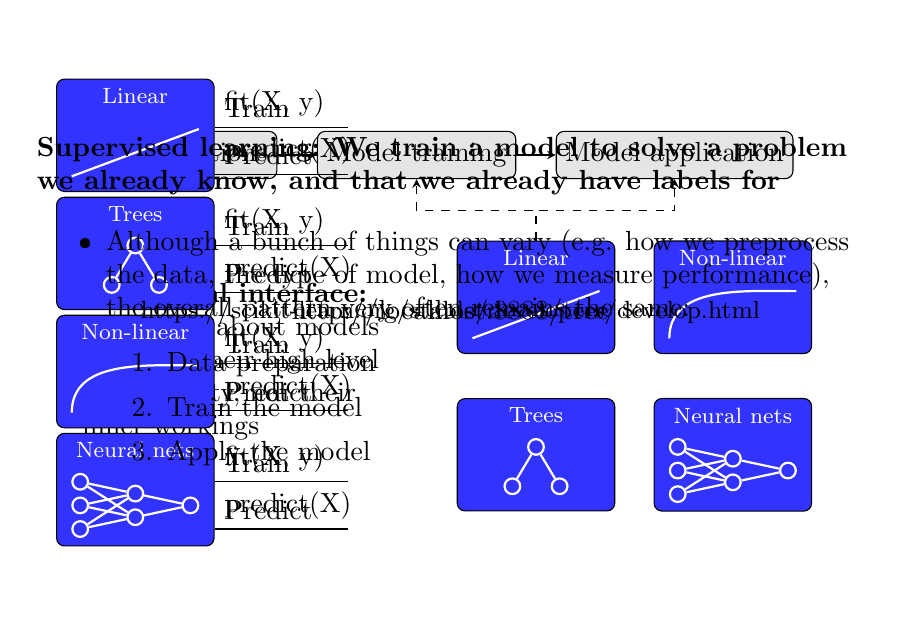
\begin{tikzpicture}
        \node[] at (-5.25, -3.5) {};
        \node[] at (5.25, 3.5) {};

        \visible<1-4>{
            \node[draw=black, fill=gray!20, minimum height=0.6cm, rounded corners=0.1cm] (prep) at (-3.3, 2) {
                Preparations
            };
            \node[draw=black, fill=gray!20, minimum height=0.6cm, rounded corners=0.1cm, anchor=west] (train) at ($ (prep.east) + (0.5, 0) $) {
                Model training
            };
            \node[draw=black, fill=gray!20, minimum height=0.6cm, rounded corners=0.1cm, anchor=west] (eval) at ($ (train.east) + (0.5, 0) $) {
                Model application
            };
            \draw[-stealth] (prep) -- (train);
            \draw[-stealth] (train) -- (eval);
        }
        \visible<2-4>{
            \node[draw=black, fill=blue!80, font=\footnotesize, text=white, rounded corners=0.1cm, text depth=1cm, minimum width=2cm] (linear) at ($ (train.south east)!0.5!(eval.south west) - (0, 1.5) $) {
                Linear
            };
            \draw[thick, white] ($ (linear.south west) + (0.2, 0.2) $) -- ($ (linear.south east) + (-0.2, 0.8) $);

            \draw[dashed, -stealth] (linear.north) |- ($ (train.south) - (0, 0.4) $) -| (train.south);
            \draw[dashed, -stealth] (linear.north) |- ($ (eval.south) - (0, 0.4) $) -| (eval.south);
        }
        \visible<3-4>{
            \node[draw=black, fill=blue!80, font=\footnotesize, text=white, rounded corners=0.1cm, text depth=1cm, minimum width=2cm] (trees) at ($ (train.south east)!0.5!(eval.south west) - (0, 3.5) $) {
                Trees
            };
            \node[circle, draw=white, thick, inner sep=2pt] (t0) at ($ (trees) + (0, 0.1) $) {};
            \node[circle, draw=white, thick, inner sep=2pt] (t1) at ($ (trees) + (0.3, -0.4) $) {};
            \node[circle, draw=white, thick, inner sep=2pt] (t2) at ($ (trees) + (-0.3, -0.4) $) {};
            \draw[thick, white] (t0) -- (t1);
            \draw[thick, white] (t0) -- (t2);

            \node[draw=black, fill=blue!80, font=\footnotesize, text=white, rounded corners=0.1cm, text depth=1cm, minimum width=2cm] (nonlinear) at ($ (train.south east)!0.5!(eval.south west) - (-2.5, 1.5) $) {
                Non-linear
            };
            \draw[thick, white] ($ (nonlinear.south west) + (0.2, 0.2) $) to [out=90, in=180] ($ (nonlinear.south east) + (-0.2, 0.8) $);
            \node[draw=black, fill=blue!80, font=\footnotesize, text=white, rounded corners=0.1cm, text depth=1cm, minimum width=2cm] (nn) at ($ (train.south east)!0.5!(eval.south west) - (-2.5, 3.5) $) {
                Neural nets
            };
            \node[circle, draw=white, thick, inner sep=2pt] (n0) at ($ (nn) + (-0.7, 0.1) $) {};
            \node[circle, draw=white, thick, inner sep=2pt] (n1) at ($ (nn) + (-0.7, -0.2) $) {};
            \node[circle, draw=white, thick, inner sep=2pt] (n2) at ($ (nn) + (-0.7, -0.5) $) {};
            \node[circle, draw=white, thick, inner sep=2pt] (n3) at ($ (nn) + (0, -0.05) $) {};
            \node[circle, draw=white, thick, inner sep=2pt] (n4) at ($ (nn) + (0, -0.35) $) {};
            \node[circle, draw=white, thick, inner sep=2pt] (n5) at ($ (nn) + (0.7, -0.2) $) {};

            \draw[thick, white] (n0) -- (n3);
            \draw[thick, white] (n0) -- (n4);
            \draw[thick, white] (n1) -- (n3);
            \draw[thick, white] (n1) -- (n4);
            \draw[thick, white] (n2) -- (n3);
            \draw[thick, white] (n2) -- (n4);
            \draw[thick, white] (n3) -- (n5);
            \draw[thick, white] (n4) -- (n5);

        }
        \visible<4>{
            \node[text width=4.3cm, align=flush left, anchor=north west] at (-4.8, 0.5) {
                \textbf{Functional interface:}\\
                We reason about models based on their high level functionality, not their inner workings
            };
        }
        \visible<5-7>{
            \node[draw=black, fill=blue!80, font=\footnotesize, text=white, rounded corners=0.1cm, text depth=1cm, minimum width=2cm] (linear) at (-4, 2.25) {
                Linear
            };
            \draw[thick, white] ($ (linear.south west) + (0.2, 0.2) $) -- ($ (linear.south east) + (-0.2, 0.8) $);

            \node[draw=black, fill=blue!80, font=\footnotesize, text=white, rounded corners=0.1cm, text depth=1cm, minimum width=2cm] (trees) at (-4, 0.75) {
                Trees
            };
            \node[circle, draw=white, thick, inner sep=2pt] (t0) at ($ (trees) + (0, 0.1) $) {};
            \node[circle, draw=white, thick, inner sep=2pt] (t1) at ($ (trees) + (0.3, -0.4) $) {};
            \node[circle, draw=white, thick, inner sep=2pt] (t2) at ($ (trees) + (-0.3, -0.4) $) {};
            \draw[thick, white] (t0) -- (t1);
            \draw[thick, white] (t0) -- (t2);

            \node[draw=black, fill=blue!80, font=\footnotesize, text=white, rounded corners=0.1cm, text depth=1cm, minimum width=2cm] (nonlinear) at (-4, -0.75) {
                Non-linear
            };
            \draw[thick, white] ($ (nonlinear.south west) + (0.2, 0.2) $) to [out=90, in=180] ($ (nonlinear.south east) + (-0.2, 0.8) $);

            \node[draw=black, fill=blue!80, font=\footnotesize, text=white, rounded corners=0.1cm, text depth=1cm, minimum width=2cm] (nn) at (-4, -2.25) {
                Neural nets
            };
            \node[circle, draw=white, thick, inner sep=2pt] (n0) at ($ (nn) + (-0.7, 0.1) $) {};
            \node[circle, draw=white, thick, inner sep=2pt] (n1) at ($ (nn) + (-0.7, -0.2) $) {};
            \node[circle, draw=white, thick, inner sep=2pt] (n2) at ($ (nn) + (-0.7, -0.5) $) {};
            \node[circle, draw=white, thick, inner sep=2pt] (n3) at ($ (nn) + (0, -0.05) $) {};
            \node[circle, draw=white, thick, inner sep=2pt] (n4) at ($ (nn) + (0, -0.35) $) {};
            \node[circle, draw=white, thick, inner sep=2pt] (n5) at ($ (nn) + (0.7, -0.2) $) {};

            \draw[thick, white] (n0) -- (n3);
            \draw[thick, white] (n0) -- (n4);
            \draw[thick, white] (n1) -- (n3);
            \draw[thick, white] (n1) -- (n4);
            \draw[thick, white] (n2) -- (n3);
            \draw[thick, white] (n2) -- (n4);
            \draw[thick, white] (n3) -- (n5);
            \draw[thick, white] (n4) -- (n5);
        }
        \visible<6>{
            \draw[] ($ (linear.east) + (0, 0.1) $) -- ++(1.3, 0);
            \node[anchor=south west] at ($ (linear.east) + (0, 0.1) $) {Train};
            \draw[] ($ (linear.east) + (0, -0.5) $) -- ++(1.3, 0);
            \node[anchor=south west] at ($ (linear.east) + (0, -0.5) $) {Predict};

            \draw[] ($ (trees.east) + (0, 0.1) $) -- ++(1.3, 0);
            \node[anchor=south west] at ($ (trees.east) + (0, 0.1) $) {Train};
            \draw[] ($ (trees.east) + (0, -0.5) $) -- ++(1.3, 0);
            \node[anchor=south west] at ($ (trees.east) + (0, -0.5) $) {Predict};

            \draw[] ($ (nonlinear.east) + (0, 0.1) $) -- ++(1.3, 0);
            \node[anchor=south west] at ($ (nonlinear.east) + (0, 0.1) $) {Train};
            \draw[] ($ (nonlinear.east) + (0, -0.5) $) -- ++(1.3, 0);
            \node[anchor=south west] at ($ (nonlinear.east) + (0, -0.5) $) {Predict};

            \draw[] ($ (nn.east) + (0, 0.1) $) -- ++(1.3, 0);
            \node[anchor=south west] at ($ (nn.east) + (0, 0.1) $) {Train};
            \draw[] ($ (nn.east) + (0, -0.5) $) -- ++(1.3, 0);
            \node[anchor=south west] at ($ (nn.east) + (0, -0.5) $) {Predict};
        }
        \visible<7>{
            \draw[] ($ (linear.east) + (0, 0.1) $) -- ++(1.7, 0);
            \node[anchor=south west] at ($ (linear.east) + (0, 0.1) $) {fit(X, y)};
            \draw[] ($ (linear.east) + (0, -0.5) $) -- ++(1.7, 0);
            \node[anchor=south west] at ($ (linear.east) + (0, -0.5) $) {predict(X)};

            \draw[] ($ (trees.east) + (0, 0.1) $) -- ++(1.7, 0);
            \node[anchor=south west] at ($ (trees.east) + (0, 0.1) $) {fit(X, y)};
            \draw[] ($ (trees.east) + (0, -0.5) $) -- ++(1.7, 0);
            \node[anchor=south west] at ($ (trees.east) + (0, -0.5) $) {predict(X)};

            \draw[] ($ (nonlinear.east) + (0, 0.1) $) -- ++(1.7, 0);
            \node[anchor=south west] at ($ (nonlinear.east) + (0, 0.1) $) {fit(X, y)};
            \draw[] ($ (nonlinear.east) + (0, -0.5) $) -- ++(1.7, 0);
            \node[anchor=south west] at ($ (nonlinear.east) + (0, -0.5) $) {predict(X)};

            \draw[] ($ (nn.east) + (0, 0.1) $) -- ++(1.7, 0);
            \node[anchor=south west] at ($ (nn.east) + (0, 0.1) $) {fit(X, y)};
            \draw[] ($ (nn.east) + (0, -0.5) $) -- ++(1.7, 0);
            \node[anchor=south west] at ($ (nn.east) + (0, -0.5) $) {predict(X)};
        }
        \visible<8>{
            \node[font=\small] at (0, 0) {
                \url{https://scikit-learn.org/stable/developers/develop.html}
            };
        }
        \visible<9>{
            \node[] at (0, 0) {
                \url{http://localhost:8888/tree}
            };
        }
        \visible<10>{
            \node[text width=10.5cm, align=flush left] at (0, 0) {
                \textbf{Supervised learning: We train a model to solve a problem we already know, and that we already have labels for}\\
                \begin{itemize}
                    \item Although a bunch of things can vary (e.g. how we preprocess the data, the type of model, how we measure performance), the overall pattern very often remains the same:
                    \begin{enumerate}
                        \item Data preparation
                        \item Train the model
                        \item Apply the model
                    \end{enumerate}
                \end{itemize}
            };
        }
    \end{tikzpicture}
\end{frame}

\begin{frame}{Introduction: Model performance}
    \begin{tikzpicture}
        \node[] at (-5.25, -3.5) {};
        \node[] at (5.25, 3.5) {};

        \visible<1-9>{
            \draw[dashed] (0, -3.5) -- (0, 3.5);
        }

        \visible<1-5>{
            \node[anchor=north] at (-2.675, 3.5) {\textbf{Regression}};
        }
        \visible<6-9>{
            \node[anchor=north,text=gray!20] at (-2.675, 3.5) {\textbf{Regression}};
        }
        \visible<1-2,6-9>{
            \node[anchor=north] at (2.675, 3.5) {\textbf{Classification}};
        }
        \visible<3-5>{
            \node[anchor=north, text=gray!20] at (2.675, 3.5) {\textbf{Classification}};
        }

        \visible<2>{
            \node[anchor=north west, ampersand replacement=\&, inner sep=0pt] (regdata) at (-5.25, 2) {
                \begin{tabular}{|c|}
                    \hline
                    $\boldsymbol{y}$\\
                    \hline
                    18\\
                    15\\
                    18\\
                    16\\
                    17\\
                    \hline
                \end{tabular}
            };
        }
        \visible<2,6>{
            \node[anchor=north west, ampersand replacement=\&, inner sep=0pt] (classdata) at (0.2, 2) {
                \begin{tabular}{|c|}
                    \hline
                    $\boldsymbol{y}$\\
                    \hline
                    cat\\
                    cat\\
                    dog\\
                    cat\\
                    dog\\
                    \hline
                \end{tabular}
            };
        }
        \visible<3-5>{
            \node[anchor=north west, ampersand replacement=\&, inner sep=0pt, text=gray!20] (classdata) at (0.2, 2) {
                \begin{tabular}{|c|}
                    \hline
                    $\boldsymbol{y}$\\
                    \hline
                    cat\\
                    cat\\
                    dog\\
                    cat\\
                    dog\\
                    \hline
                \end{tabular}
            };

            \node[anchor=north west, ampersand replacement=\&, inner sep=0pt] (regdata) at (-5.25, 2) {
                \begin{tabular}{|c|c|}
                    \hline
                    $\boldsymbol{y}$&$\boldsymbol{\hat{y}}$\\
                    \hline
                    18&15.3\\
                    15&16.1\\
                    18&17.2\\
                    16&16.8\\
                    17&19.5\\
                    \hline
                \end{tabular}
            };
        }
        \visible<4-5>{
            \node[anchor=north, text width=5cm, align=center, text depth=0] at (-2.675, -2) {
                \underline{\textbf{Mean squared error (MSE):}}\\
                $\dfrac{1}{n}\sum_{i=0}^n(y_i-\hat{y}_i)^2$
            };
        }
        \visible<5>{
            \node[anchor=south west, ampersand replacement=\&, text=red, inner sep=0pt] (regloss) at (regdata.south east) {
                \begin{tabular}{c}
                    $(18-15.3)^2=7.29$\\
                    $(15-16.1)^2=1.21$\\
                    $(18-17.2)^2=0.64$\\
                    $(16-16.4)^2=0.16$\\
                    $(17-19.5)^2=6.25$\\
                \end{tabular}
            };
            \draw[red, thick] ($ (regloss.south east) - (0.2, -0.06) $) -- ++(-0.7, 0);
            \node[text=red, anchor=north east, inner sep=0pt] at ($ (regloss.south east) - (0.26, 0.1) $) {
                $\mathbf{3.11}$
            };
        }
        \visible<6-9>{
            \node[anchor=north west, ampersand replacement=\&, inner sep=0pt, text=gray!20] (regdata) at (-5.25, 2) {
                \begin{tabular}{|c|c|}
                    \hline
                    $\boldsymbol{y}$&$\boldsymbol{\hat{y}}$\\
                    \hline
                    18&15.3\\
                    15&16.1\\
                    18&17.2\\
                    16&16.8\\
                    17&19.5\\
                    \hline
                \end{tabular}
            };
            \node[anchor=north, text width=5cm, align=center, text depth=0, text=gray!20] at (-2.675, -2) {
                \underline{\textbf{Mean squared error (MSE):}}\\
                $\dfrac{1}{n}\sum_{i=0}^n(y_i-\hat{y}_i)^2$
            };
            \node[anchor=south west, ampersand replacement=\&, text=red!20, inner sep=0pt] (regloss) at (regdata.south east) {
                \begin{tabular}{c}
                    $(18-15.3)^2=7.29$\\
                    $(15-16.1)^2=1.21$\\
                    $(18-17.2)^2=0.64$\\
                    $(16-16.4)^2=0.16$\\
                    $(17-19.5)^2=6.25$\\
                \end{tabular}
            };
            \draw[red!20, thick] ($ (regloss.south east) - (0.2, -0.06) $) -- ++(-0.7, 0);
            \node[text=red!20, anchor=north east, inner sep=0pt] at ($ (regloss.south east) - (0.26, 0.1) $) {
                $\mathbf{3.11}$
            };
        }
        \visible<7-9>{
            \node[anchor=north west, ampersand replacement=\&, inner sep=0pt] (classdata) at (0.2, 2) {
                \begin{tabular}{|c|c|}
                    \hline
                    $\boldsymbol{y}$&$\boldsymbol{\hat{y}}$\\
                    \hline
                    cat&cat\\
                    cat&dog\\
                    dog&dog\\
                    cat&cat\\
                    dog&cat\\
                    \hline
                \end{tabular}
            };
        }
        \visible<8-9>{
            \node[anchor=north, text width=5cm, align=center, text depth=0] at (2.675, -2) {
                \underline{\textbf{Accuracy:}}\\
                $\dfrac{1}{n}\sum_{i=0}^n \mathds{1}(y=\hat{y})$
            };
        }
        \visible<9>{
            \node[anchor=south west, ampersand replacement=\&, text=red, inner sep=0pt] (classloss) at (classdata.south east) {
                \setlength{\tabcolsep}{0pt}
                \begin{tabular}{ll}
                    cat$=$cat&$\implies$1\\
                    cat$\neq$dog&$\implies$0\\
                    dog$=$dog&$\implies$1\\
                    cat$=$cat&$\implies$1\\
                    dog$\neq$cat&$\implies$0\\
                \end{tabular}
            };
            \draw[red, thick] ($ (classloss.south east) - (-0.25, -0.06) $) -- ++(-0.7, 0);
            \node[text=red, anchor=north east, inner sep=0pt] at ($ (classloss.south east) - (-0.25, 0.1) $) {
                $\mathbf{0.60}$
            };
        }
        \only<10,13>{
            \node[] at (0, 0) {
                \url{http://localhost:8888/tree}
            };
        }
        \only<11-12>{
            \node[] at (0, 1) {
                mean\_squared\_error(y, predictions)
            };
        }
        \only<12>{
            \node[] at (0, 0.5) {
                mean\_absolute\_error(y, predictions)
            };
            \node[] at (0, 0) {
                median\_absolute\_error(y, predictions)
            };
            \node[] at (0, -0.5) {
                r2\_score(y, predictions)
            };
            \node[] at (0, -1) {
                \vdots
            };

            \node[font=\small] at (0, -3) {
                \url{https://scikit-learn.org/stable/api/sklearn.metrics.html}
            };
        }
        \visible<14>{
            \node[text width=10.5cm, align=flush left] at (0, 0) {
                \textbf{We generally divide prediction problems into two types, regression and classification}
                \begin{itemize}
                    \item Regression problems deal with continuous outputs
                    \item Classification problems deal with categorical outputs
                    \item There is a range of metrics to evaluate model performance, each suitable for different purposes
                \end{itemize}
            };
        }
    \end{tikzpicture}
\end{frame}

\newcommand{\biasvarianceplot}[3]{
    \begin{tikzpicture}
        \begin{axis}[
            height=3.7cm,
            width=5.3cm,
            ylabel=$y$,
            xlabel=$x$,
            title=\textbf{#3},
            title style={
                yshift=-0.2cm,
                text depth=0,
            },
            ytick pos=left,
            xtick pos=bottom,
            xmin=0,
            xmax=100
        ]

        \addplot[
            only marks,
            color=cyan,
            opacity=0.25
        ] table [
            col sep=comma,
            x=x,
            y=y
        ] {data/bias-variance-#1.csv};
        \addplot[
            very thick,
            domain=-5:105,
            samples=100,
        ] {-0.000226*x*x*x+0.032262*x*x-1.3543*x+30};

        \ifnum#2>0
            \addplot[
                very thick,
                color=purple
            ] table [
                col sep=comma,
                x=x,
                y=linear_y
            ] {data/bias-variance-#1.csv};
        \fi
        \ifnum#2>1
            \addplot[
                very thick,
                color=orange
            ] table [
                col sep=comma,
                x=x,
                y=polynomial_y
            ] {data/bias-variance-#1.csv};
        \fi

        \end{axis}
    \end{tikzpicture}
}
\newsavebox{\biasvariancetraindata}
\sbox{\biasvariancetraindata}{
    \biasvarianceplot{train}{0}{Training data}
}
\newsavebox{\biasvariancetestdata}
\sbox{\biasvariancetestdata}{
    \biasvarianceplot{test}{0}{Test data}
}
\newsavebox{\biasvariancetrainlinear}
\sbox{\biasvariancetrainlinear}{
    \biasvarianceplot{train}{1}{Training data}
}
\newsavebox{\biasvariancetestlinear}
\sbox{\biasvariancetestlinear}{
    \biasvarianceplot{test}{1}{Test data}
}
\newsavebox{\biasvariancetrainpolynomial}
\sbox{\biasvariancetrainpolynomial}{
    \biasvarianceplot{train}{2}{Training data}
}
\newsavebox{\biasvariancetestpolynomial}
\sbox{\biasvariancetestpolynomial}{
    \biasvarianceplot{test}{2}{Test data}
}

\newcommand{\residualplot}[5]{
    \begin{tikzpicture}
        \begin{axis}[
            height=3.7cm,
            width=5.3cm,
            ylabel=$y-\hat{y}$,
            xlabel=$x$,
            title=\textbf{#3},
            title style={
                yshift=-0.2cm,
                text depth=0,
            },
            ytick pos=left,
            xtick pos=bottom,
            xmin=0,
            xmax=100,
            ymin=-#5,
            ymax=#5,
            ylabel style={
                yshift=-0.17cm
            }
        ]

        \addplot[
            only marks,
            color=cyan,
            opacity=0.25
        ] table [
            col sep=comma,
            x=x,
            y=#2_residuals
        ] {data/bias-variance-#1.csv};

        \draw[thick, #4] (axis cs: 0, 0) -- (axis cs: 100, 0);

        \end{axis}
    \end{tikzpicture}
}

\newsavebox{\residualtrainlinear}
\sbox{\residualtrainlinear}{
    \residualplot{train}{linear}{Simple model (train)}{purple}{20}
}
\newsavebox{\residualtestlinear}
\sbox{\residualtestlinear}{
    \residualplot{test}{linear}{Simple model (test)}{purple}{20}
}
\newsavebox{\residualtrainpolynomial}
\sbox{\residualtrainpolynomial}{
    \residualplot{train}{polynomial}{Complex model (train)}{orange}{6}
}
\newsavebox{\residualtestpolynomial}
\sbox{\residualtestpolynomial}{
    \residualplot{test}{polynomial}{Complex model (test)}{orange}{6}
}

\newcommand{\tradeoffplot}[1]{
    \begin{tikzpicture}
        \begin{axis}[
            height=6cm,
            width=9cm,
            ymajorticks=false,
            xmajorticks=false,
            ylabel=Model error,
            xlabel=Flexibility,
            axis lines=left,
            xmin=0,
            xmax=1,
            ymin=0,
            ymax=2.5,
            clip=false
        ]
            \node[] at (axis cs: 1.34, 2.9) {};

            \ifnum#1>0
                \draw[dotted] (axis cs: 0.1, 0) -- (axis cs: 0.1, 2.5);
                \node[anchor=south, align=center, font=\footnotesize\linespread{0.9}\selectfont] at (axis cs: 0.1, 2.5) {
                    Simple\\model
                };
                \addplot[
                    only marks,
                    mark options={
                        draw=black,
                        fill=bias,
                        scale=2
                    }
                ] coordinates {
                    (0.1, 0.5)
                    (1.05, 2.4)
                };
                \node[anchor=west] at (axis cs: 1.065, 2.4) {
                    Bias
                };

                \addplot[
                    only marks,
                    mark options={
                        draw=black,
                        fill=variance,
                        scale=2
                    }
                ] coordinates {
                    (0.1, 0.01114)
                    (1.05, 2.2)
                };
                \node[anchor=west] at (axis cs: 1.065, 2.2) {
                    Variance
                };
            \fi
            \ifnum#1>1
                \draw[dotted] (axis cs: 0.75, 0) -- (axis cs: 0.75, 2.5);
                \node[anchor=south, align=center, font=\footnotesize\linespread{0.9}\selectfont] at (axis cs: 0.75, 2.5) {
                    Complex\\model
                };
                \addplot[
                    only marks,
                    mark options={
                        draw=black,
                        fill=bias,
                        scale=2
                    }
                ] coordinates {
                    (0.75, 0.117)
                };

                \addplot[
                    only marks,
                    mark options={
                        draw=black,
                        fill=variance,
                        scale=2
                    }
                ] coordinates {
                    (0.75, 0.2873)
                };
            \fi
            \ifnum#1>2
                \addplot[
                    bias,
                    very thick,
                    domain=0:1,
                    samples=100
                ] {(1/(x+0.1))/10};
                \addplot[
                    variance,
                    very thick,
                    domain=0:1,
                    samples=100
                ] {(exp(x*5))/148};
            \fi
            \ifnum#1>3
                \draw[dashed] (axis cs: 0, 1.2) -- (axis cs: 1, 1.2);
                \node[anchor=west, align=left, font=\footnotesize\linespread{0.9}\selectfont] at (axis cs: 1, 1.2) {
                    Irreducible\\error
                };
            \fi
            \ifnum#1>4
                \addplot[
                    full,
                    very thick,
                    domain=0:1,
                    samples=100
                ] {((1/(x+0.1))/10) + ((exp(x*5))/148) + 1.2};

                \addplot[
                    only marks,
                    mark options={
                        draw=black,
                        fill=full,
                        scale=2
                    }
                ] coordinates {
                    (0.1, 1.71114)
                    (0.75, 1.6043)
                    (1.05, 2)
                };
                \ifnum#1<6
                    \node[anchor=west] at (axis cs: 1.065, 2) {
                        Total
                    };
                \fi
            \fi
            \ifnum#1>5
                \addplot[
                    train,
                    very thick,
                    domain=0:1,
                    samples=100
                ] {((1/(x+0.1))/10) + 1.2};

                \node[anchor=west] at (axis cs: 1.065, 2) {
                    Total (test)
                };

                \addplot[
                    only marks,
                    mark options={
                        draw=black,
                        fill=train,
                        scale=2
                    }
                ] coordinates {
                    (0.1, 1.7)
                    (0.75, 1.317)
                    (1.05, 1.8)
                };
                \node[anchor=west] at (axis cs: 1.065, 1.8) {
                    Total (train)
                };
            \fi

        \end{axis}
    \end{tikzpicture}
}

\newsavebox{\tradeoffempty}
\sbox{\tradeoffempty}{
    \tradeoffplot{0}
}
\newsavebox{\tradeoffsimple}
\sbox{\tradeoffsimple}{
    \tradeoffplot{1}
}
\newsavebox{\tradeoffcomplex}
\sbox{\tradeoffcomplex}{
    \tradeoffplot{2}
}
\newsavebox{\tradeofftraces}
\sbox{\tradeofftraces}{
    \tradeoffplot{3}
}
\newsavebox{\tradeoffirreducible}
\sbox{\tradeoffirreducible}{
    \tradeoffplot{4}
}
\newsavebox{\tradeoffloss}
\sbox{\tradeoffloss}{
    \tradeoffplot{5}
}
\newsavebox{\tradeofftrain}
\sbox{\tradeofftrain}{
    \tradeoffplot{6}
}


\begin{frame}{Introduction: The Bias-Variance Trade-off}
    \begin{tikzpicture}
        \node[] at (-5.25, -3.5) {};
        \node[] at (5.25, 3.5) {};

        \visible<1>{
            \node[inner sep=0pt, draw=black] at (0, 0) {
                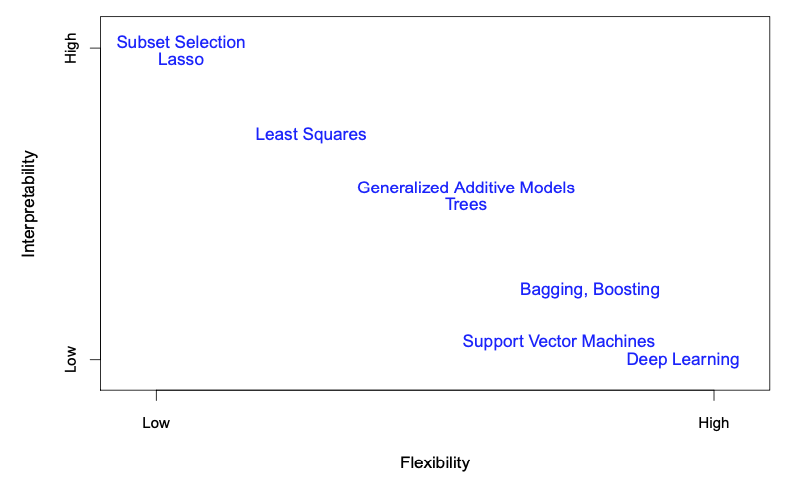
\includegraphics[width=9cm]{data/flexibility}
            };
        }
        \visible<2>{
            \node[] at (0, 1.75) {
                \usebox{\mpglinear}
            };
            \node[] at (0, -1.75) {
                \usebox{\mpgsquared}
            };
        }
        \visible<3>{
            \node[text width=10.5cm, align=flush left] at (0, 0) {
                \textbf{Model performance will depend on the dataset we use to calculate the performance metrics}
                \begin{itemize}
                    \item Training set: The data we use to estimate the model
                    \begin{itemize}
                        \item With a sufficiently flexible model we can \textbf{always} achieve 0 error in the training set
                    \end{itemize}
                    \item Test set: Data held-out from the training set such that it remains unseen by the model
                    \begin{itemize}
                        \item Performance in the test set is indicative of how well the model generalizes to new data (almost always worse than in the training set)
                        \item If our model performs well in new data, we can assume that it accurately describes the relationship between the predictors and the response in the \textbf{general case}
                    \end{itemize}
                \end{itemize}
            };
        }
        \visible<4>{
            \node[text width=10.5cm] at (0, 0) {
                \textbf{How can our model perform poorly?}
                \begin{itemize}
                    \item \underline{Underfitting}: The model is too simple to capture the relationship between the predictors and the response
                    \begin{itemize}
                        \item High error in both the training and test set
                    \end{itemize}
                    \item \underline{Overfitting}: The model is too complex and captures noise in the training set
                    \begin{itemize}
                        \item Low error in the training set, high error in the test set
                    \end{itemize}
                \end{itemize}
            };
        }
        \visible<5>{
            \node[inner sep=0pt, draw=black] at (0, 0) {
                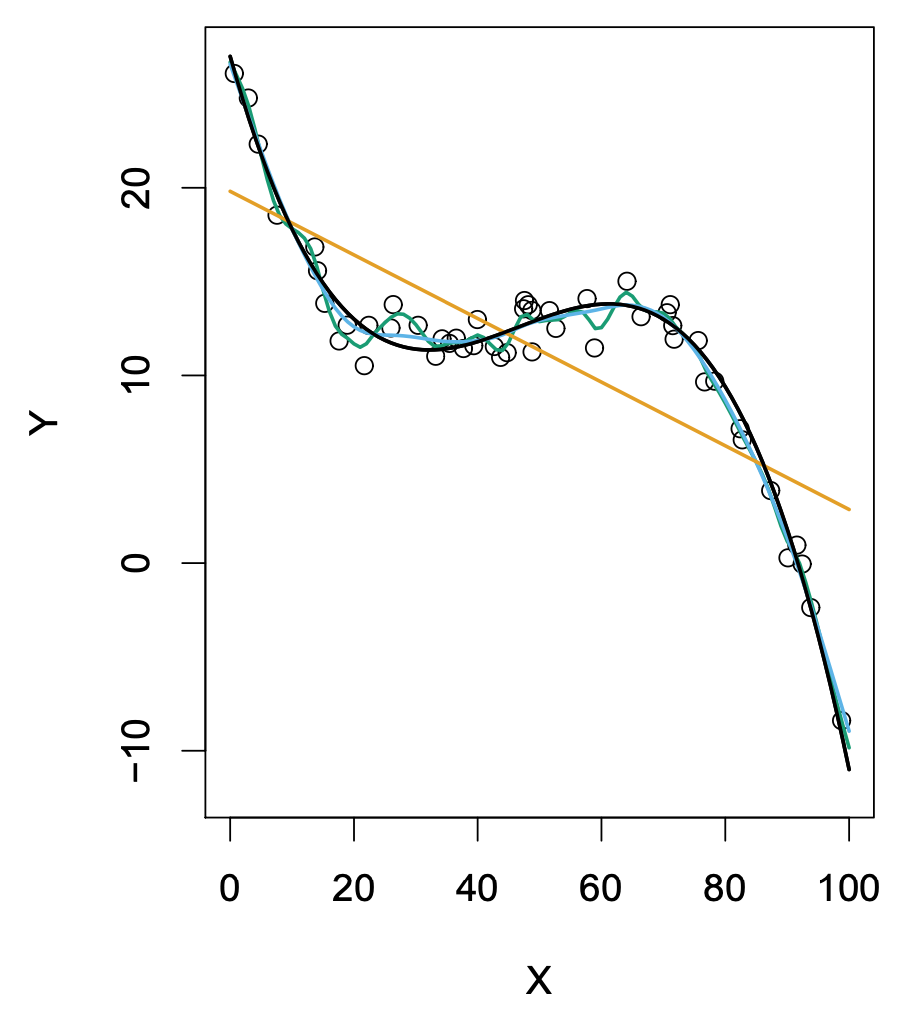
\includegraphics[width=5cm]{data/overfitting_underfitting.png}
            };
        }
        \visible<6-8>{
            \node[] (formula) at (0, 0) {
                $\mathbb{E}\left[\left(y-\hat{f}(x)\right)^2\right]=\mathrm{Var}(\hat{f}(x)) + \left[\mathrm{Bias}(\hat{f}(x))\right]^2+\mathrm{Var}(\epsilon)$
            };
        }
        \visible<7>{
            \node[text=red] (irreducible) at ($ (formula.south) + (3.6, -0.5) $) {
                Irreducible error
            };
            \draw[-stealth, red] (irreducible.north) -- ++(0, 0.5);
        }
        \visible<8>{
            \node[text=red] (bias) at ($ (formula.south) + (1.6, -0.5) $) {
                Bias
            };
            \draw[-stealth, red] (bias.north) -- ++(0, 0.5);

            \node[text=red] (variance) at ($ (formula.south) + (-0.4, -0.5) $) {
                Variance
            };
            \draw[-stealth, red] (variance.north) -- ++(0, 0.5);
        }
        \visible<9-10>{
            \node[] at (-2.675, 1.75) {
                \usebox{\biasvariancetraindata}
            };
        }
        \visible<9-12>{
            \node[font=\footnotesize, text=cyan] at (0, -0.5) {
                $f(x) = -0.000226x^3+0.032262x^2-1.3543x+30+\epsilon$
            };
        }
        \visible<10>{
            \node[] at (2.675, 1.75) {
                \usebox{\biasvariancetestdata}
            };
        }
        \visible<11>{
            \node[] at (-2.675, 1.75) {
                \usebox{\biasvariancetrainlinear}
            };
            \node[] at (2.675, 1.75) {
                \usebox{\biasvariancetestlinear}
            };
        }
        \visible<11-12>{
            \node[font=\footnotesize, text=purple] at (0, -1) {
                $\hat{f}_0(x) = -0.17x+21.74$
            };
        }
        \visible<12-15>{
            \node[] at (-2.675, 1.75) {
                \usebox{\biasvariancetrainpolynomial}
            };
            \node[] at (2.675, 1.75) {
                \usebox{\biasvariancetestpolynomial}
            };
        }
        \visible<12>{
            \node[font=\footnotesize, text=orange] at (0, -1.5) {
                $\hat{f}_1(x) = 1.32*10^{-142}x^{80}-2.18*10^{-140}x^{79}+\ldots$
            };
        }
        \visible<13>{
            \node[] at (-2.675, -1.75) {
                \usebox{\residualtrainlinear}
            };
            \node[] at (2.675, -1.75) {
                \usebox{\residualtestlinear}
            };
        }
        \visible<14>{
            \node[] at (-2.675, -1.75) {
                \usebox{\residualtrainpolynomial}
            };
            \node[] at (2.675, -1.75) {
                \usebox{\residualtestpolynomial}
            };
        }
        \visible<15>{
            \node[] at (-2.675, -1.75) {
                \usebox{\residualtestlinear}
            };
            \node[] at (2.675, -1.75) {
                \usebox{\residualtestpolynomial}
            };
        }
        \visible<16>{
            \node[] at (0, 0.5) {
                \usebox{\tradeoffempty}
            };
        }
        \visible<17>{
            \node[] at (0, 0.5) {
                \usebox{\tradeoffsimple}
            };
        }
        \visible<18>{
            \node[] at (0, 0.5) {
                \usebox{\tradeoffcomplex}
            };
        }
        \visible<19-20>{
            \node[] at (0, 0.5) {
                \usebox{\tradeofftraces}
            };
        }
        \visible<20-21>{
            \node[] (formula) at (0, -2.95) {
                $\mathbb{E}\left[\left(y-\hat{f}(x)\right)^2\right]={\color{variance}\mathrm{Var}(\hat{f}(x))} + {\color{bias}\left[\mathrm{Bias}(\hat{f}(x))\right]^2}+\mathrm{Var}(\epsilon)$
            };
        }
        \visible<21>{
            \node[] at (0, 0.5) {
                \usebox{\tradeoffirreducible}
            };
        }
        \visible<22>{
            \node[] at (0, 0.5) {
                \usebox{\tradeoffloss}
            };
            \node[] (formula) at (0, -2.95) {
                ${\color{full}\mathbb{E}\left[\left(y-\hat{f}(x)\right)^2\right]}={\color{variance}\mathrm{Var}(\hat{f}(x))} + {\color{bias}\left[\mathrm{Bias}(\hat{f}(x))\right]^2}+\mathrm{Var}(\epsilon)$
            };
        }
        \visible<23-24>{
            \node[] at (0, 0.5) {
                \usebox{\tradeofftrain}
            };
        }
        \visible<24>{
            \draw[stealth-stealth, line width=4pt] (-4.6, 0.25) -- (2.7, 0.25);
            \node[font=\bfseries, anchor=north west, draw=black, fill=white, text depth=0] at (-4.6, -0.05) {
                \textbf{Underfitting}
            };
            \node[font=\bfseries, anchor=north east, draw=black, fill=white, text depth=0] at (2.7, -0.05) {
                \textbf{Overfitting}
            };
        }
        \visible<25>{
            \node[text width=10.5cm, align=flush left] at (0, 0) {
                \textbf{The bias-variance trade-off lets us reason about why our model performs poorly}
                \begin{itemize}
                    \item If our model is too simple it will have high bias and low variance, which we can recognize by a high error in both the training and test set
                    \item If our model is too complex it will have low bias and high variance, which we can recognize by a low error in the training set and a high error in the test set
                    \item \textbf{This is way easier in theory than in practice}
                \end{itemize}
            };
        }
    \end{tikzpicture}
\end{frame}

\newsavebox{\groundtruth}
\sbox{\groundtruth}{
    \begin{tikzpicture}
        \begin{axis}[
            height=6cm,
            width=9cm,
            ylabel=$y$,
            xlabel=$x$,
            title style={
                yshift=-0.2cm,
                text depth=0,
            },
            ytick pos=left,
            xtick pos=bottom,
            xmin=0,
            xmax=100
        ]

            \addplot[
                only marks,
                color=cyan,
                opacity=0.25
            ] table [
                col sep=comma,
                x=x,
                y=y
            ] {data/bias-variance-train.csv};
            \addplot[
                very thick,
                domain=-5:105,
                samples=100,
            ] {-0.000226*x*x*x+0.032262*x*x-1.3543*x+30};
        \end{axis}
    \end{tikzpicture}
}

\newcommand{\classificationplot}[1]{
    \begin{tikzpicture}
        \begin{axis}[
            height=6cm,
            width=6cm,
            xlabel=$x_1$,
            ylabel=$x_2$,
            xtick pos=bottom,
            ytick pos=left,
            xmin=-0.99,
            xmax=1.3,
            ymin=-0.65,
            ymax=1.35
        ]
            \ifnum#1=0
                \addplot[
                    only marks,
                    draw=gray,
                    opacity=0.5
                ] table [
                    col sep=comma,
                    x=x1,
                    y=x2
                ] {data/bayesdata.csv};
            \fi

            \ifnum#1>0
                \addplot[
                    only marks,
                    red,
                    opacity=0.5,
                    discard if not={y}{0.0}
                ] table [
                    col sep=comma,
                    x=x1,
                    y=x2
                ] {data/bayesdata.csv};
                \addplot[
                    only marks,
                    blue,
                    opacity=0.5,
                    discard if not={y}{1.0}
                ] table [
                    col sep=comma,
                    x=x1,
                    y=x2
                ] {data/bayesdata.csv};
            \fi

            \ifnum#1=2
                \draw[dashed, thick] (axis cs: -0.6, 1.35) -- (axis cs: 0.8, -0.65);
                \node[anchor=north west, rotate=302, font=\footnotesize\linespread{0.85}\selectfont\bfseries, align=center] at (axis cs: -0.55, 1.35) {
                    Decision\\boundary
                };
            \fi

            \ifnum#1=3
                \addplot [smooth, thick, dashed] coordinates {
                    (-0.3, 1.35)
                    (0.2, 0.2)
                    (0.4, -0.2)
                    (1.6, -0.65)
                };
            \fi
        \end{axis}
    \end{tikzpicture}
}

\newsavebox{\classificationpoints}
\sbox{\classificationpoints}{
    \classificationplot{0}
}
\newsavebox{\classificationclasses}
\sbox{\classificationclasses}{
    \classificationplot{1}
}
\newsavebox{\classificationboundary}
\sbox{\classificationboundary}{
    \classificationplot{2}
}
\newsavebox{\classificationbayes}
\sbox{\classificationbayes}{
    \classificationplot{3}
}

\begin{frame}{Introduction: The Bayes Classifier}
    \begin{tikzpicture}
        \node[] at (-5.25, -3.5) {};
        \node[] at (5.25, 3.5) {};

        \visible<1>{
            \node[] at (0, 0.5) {
                \usebox{\groundtruth}
            };
            \node[] at (0, -2.5) {
                $y=f(x)+\epsilon$
            };
        }
        \visible<2>{
            \node[inner sep=0pt, draw=black, anchor=west] (x1) at (-5.25, 2.5) {
                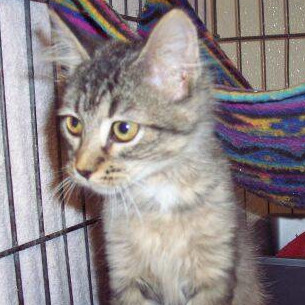
\includegraphics[width=1cm]{data/cats_and_dogs/cat.2.jpg}
            };
            \node[inner sep=0pt, draw=black] (x2) at ($ (x1) - (0, 1.5) $) {
                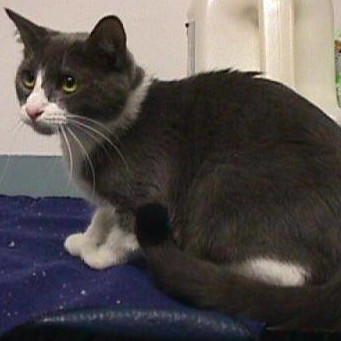
\includegraphics[width=1cm]{data/cats_and_dogs/cat.0.jpg}
            };
            \node[inner sep=0pt, draw=black] (x3) at ($ (x1) - (0, 3) $) {
                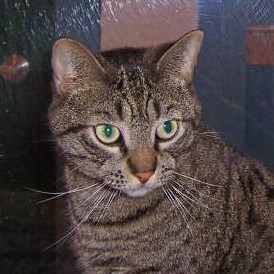
\includegraphics[width=1cm]{data/cats_and_dogs/cat.1.jpg}
            };
            \node[inner sep=0pt, draw=black] (x3) at ($ (x1) - (0, 4.5) $) {
                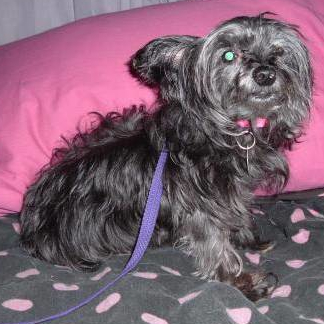
\includegraphics[width=1cm]{data/cats_and_dogs/dog.0.jpg}
            };

            \node[inner sep=0pt, draw=black] (x5) at ($ (x1) - (-1.25, 0.75) $) {
                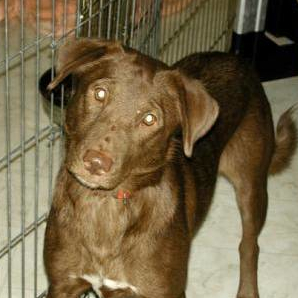
\includegraphics[width=1cm]{data/cats_and_dogs/dog.1.jpg}
            };
            \node[inner sep=0pt, draw=black] (x6) at ($ (x1) - (-1.25, 2.25) $) {
                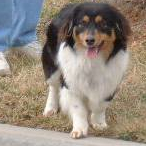
\includegraphics[width=1cm]{data/cats_and_dogs/dog.2.jpg}
            };
            \node[inner sep=0pt, draw=black] (x7) at ($ (x1) - (-1.25, 3.75) $) {
                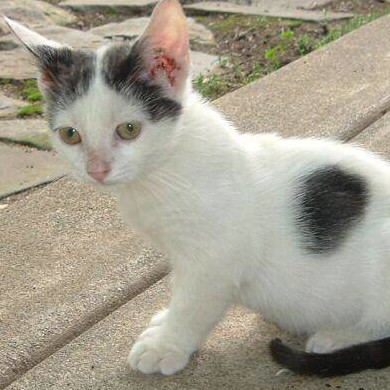
\includegraphics[width=1cm]{data/cats_and_dogs/cat.3.jpg}
            };
            \node[align=center, font=\scriptsize, draw=black] (sm) at ($ (x6) + (2.3, 0) $) {
                Supervised\\model
            };

            \draw[-stealth, gray!50, line width=3pt] (x6) to (sm);
            \draw[-stealth, gray!50, line width=3pt] (sm) -- ($ (sm.east) + (1.1, 0) $);

            \node[inner sep=0pt, draw=black] (y1) at ($ (sm.center) + (5, 0.5) $) {
                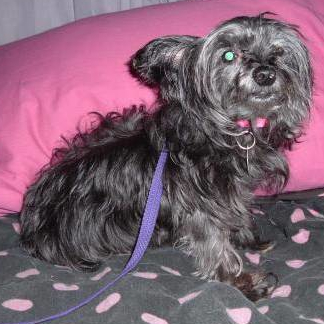
\includegraphics[width=1cm]{data/cats_and_dogs/dog.0.jpg}
            };
            \node[anchor=west, inner sep=0pt, draw=black] (y2) at (y1.east) {
                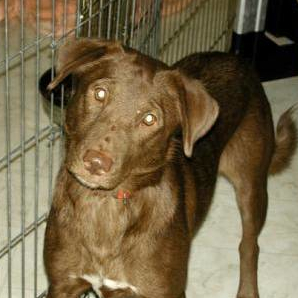
\includegraphics[width=1cm]{data/cats_and_dogs/dog.1.jpg}
            };
            \node[anchor=north, inner sep=0pt, draw=black] at (y1.south) {
                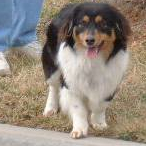
\includegraphics[width=1cm]{data/cats_and_dogs/dog.2.jpg}
            };

            \node[inner sep=0pt, draw=black] (y4) at ($ (sm) + (2.5, 0.5) $) {
                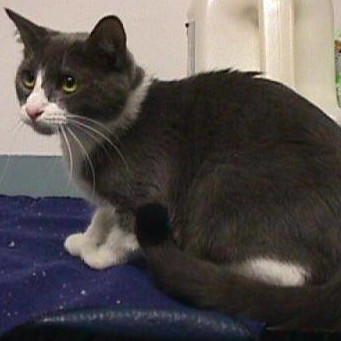
\includegraphics[width=1cm]{data/cats_and_dogs/cat.0.jpg}
            };
            \node[anchor=west, inner sep=0pt, draw=black] (y5) at (y4.east) {
                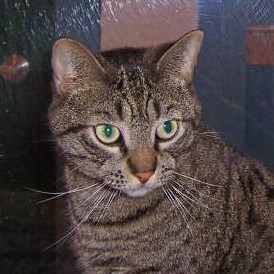
\includegraphics[width=1cm]{data/cats_and_dogs/cat.1.jpg}
            };
            \node[anchor=north, inner sep=0pt, draw=black] (y6) at (y4.south) {
                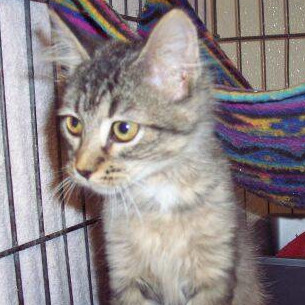
\includegraphics[width=1cm]{data/cats_and_dogs/cat.2.jpg}
            };
            \node[anchor=north, inner sep=0pt, draw=black] (y7) at (y5.south) {
                \includegraphics[width=1cm]{data/cats_and_dogs/cat.3.jpg}
            };

            \node[anchor=south, text depth=0] at ($ (y1.north)!0.5!(y2.north) $) {
                Dogs
            };
            \node[anchor=south, text depth=0] at ($ (y4.north)!0.5!(y5.north) $) {
                Cats
            };
        }
        \visible<3-7>{
            \node[ampersand replacement=\&] at (-2.75, 0.5) {
                \begin{tabular}{|c|c|c|}
                    \hline
                    $\mathbf{x_1}$&$\mathbf{x_2}$&$\mathbf{y}$\\
                    \hline
                    -0.06&0.17&0\\
                    1.16&1.20&1\\
                    1.12&1.60&1\\
                    0.69&0.28&0\\
                    1.25&1.11&1\\
                    \hline
                \end{tabular}
            };
        }
        \visible<4>{
            \node[] at (2.25, 0.5) {
                \usebox{\classificationpoints}
            };
        }
        \visible<5>{
            \node[] at (2.25, 0.5) {
                \usebox{\classificationclasses}
            };
        }
        \visible<6>{
            \node[] at (2.25, 0.5) {
                \usebox{\classificationboundary}
            };
        }
        \visible<7>{
            \node[] at (2.25, 0.5) {
                \usebox{\classificationbayes}
            };
            \node[] at (2.75, -2.75) {
                $y=\underset{k\in\{0,1\}}{\mathrm{argmax}}\ Pr(y=k|x)$
            };
        }
        \visible<8>{
            \node[text width=10.5cm] at (0, 0) {
                \textbf{Classification can be seen as the task of finding a decision boundary that best separates our classes in a high-dimensional vector space representing our predictors}
                \begin{itemize}
                    \item The Bayes classifier is the best classifier that can be theoretically achieved (although in practice we have to approimate it using data)
                    \item The Bayes error rate quantifies the error of the best possible classifier
                \end{itemize}
            };
        }
    \end{tikzpicture}
\end{frame}

\begin{frame}{Assignment 1}
    Follow the steps in Chapter 2.3 of Introduction to Statistical Learning to make sure your system is set up correctly, whether you want to use Python or R. Then do the following exercises to make sure you understand:

    \begin{itemize}
        \item Create a vector of 100 standard normally distributed numbers and visualize them with a histogram.
        \item Show rows 5, 8, 9, and 10 of the Auto dataset.
        \item Show the last three columns of the Auto dataset.
        \item Show all cars with five cylinders in the Auto dataset.
    \end{itemize}
\end{frame}

\end{document}
